\newpage
\hypertarget{rules common}{}
\subsection{Implementing IndexToLevel}
\genHeader

If you have done everything right up to this point, your project should save and build without error in Eclipse. In fact, there should now be three
generated repository projects included in \texttt{MyWorkingSet}. We're most concerned with \texttt{LearningBox\-To\-Dictionary\-Integration}, which implements
our TGG and its rules. Your folder should resemble Fig.~\ref{fig:tggGenerated}


\begin{figure}[htbp]
\begin{center}
  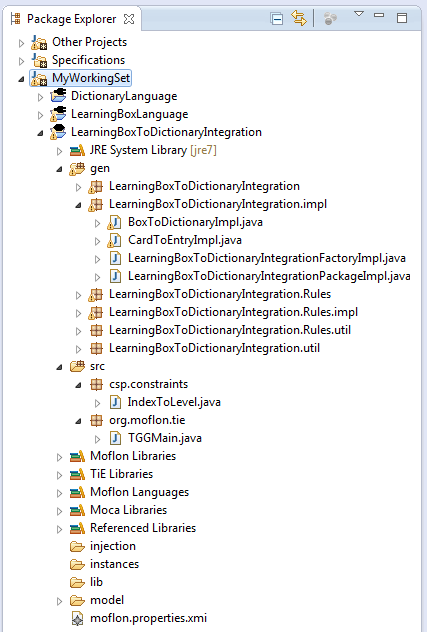
\includegraphics[width=0.7\textwidth]{eclipse_generatedTGG}
  \caption{generated stuff}
  \label{fig:tggGenerated}
\end{center}
\end{figure}

Despite all these files, our TGG isn't yet complete. While we set up and used the \texttt{IndexTolevel} attribute constraint, we haven't actually given it any
implementation code yet. Let's quickly review each constraint before we do.

Just like patterns describing \emph{structural} correspondence, \emph{attribute constraints} can be automatically \emph{operationalized} as required for
the forward concrete transformations. Even more interesting, a set of constraints might have to be ordered in a specific way depending on
the direction of the transformation, or they might have to be checked for pre-existing attributes. Others still might have to set values appropriately in
order to fulfill the constraint.

For built-in \emph{library} constraints such as \emph{eq}, \emph{addPrefix} and \emph{concat}, you do not need to worry about these details and can just focus
on expressing what should happen. Everything else is handled automatically.

In many cases however, a required constraint might be extremely narrow and problem-specific, such as our \emph{IndexToLevel}. There might not be any
fitting combination of library constraints to express the consistency condition so a new attribute constraint type must be declared before its use.

There is a list of \emph{adornments} in the declaration which specify the cases for which the constraint can be operationalized. Each adornment consists of a
\texttt{B} (bound) or \texttt{F} (free) variable setting for each argument of the constraint. It sounds complex, but is really quite simple, especially in
the context of our example:

\begin{description}

\item[BB] indicates that the \texttt{partition.index} and \texttt{entry.level} are both \emph{bound}, i.e., they already have assigned values.
In this case, the \emph{operation} must check if the assigned values are valid and correct.

\item[BF] indicates that \texttt{partition.index} is \emph{bound} and \texttt{entry.level} is \emph{free}, i.e., the operation must determine and assign the
correct value to \texttt{entry.level} using \texttt{partition.index}.

\item[FB] indicates that \texttt{partition.index} is \emph{free} and \texttt{entry.level} is \emph{bound}, i.e., the operation must determine and assign the
correct value to \texttt{parti\-tion.in\-dex} using \texttt{entry.level}.

\end{description}

Note that we decide not to support \textbf{FF} as we would have to generate a consistent pair of \texttt{index} and \texttt{level}. Although this is possible
and might even make sense for some applications, it does not in the context of partitions and entries (the pairs are not unique, so which pair should we
take? \texttt{partition2} set to \texttt{beginner}?).

At compile time, the set of constraints (also called \emph{Constraint Satisfaction Problem} (CSP)) for every TGG rule is ``solved'' for each case by
operationalizing all constraints and determining a feasible sequence in which the operations can be executed, compatible to the declared adornments of each
constration. If the constraints cannot be solved, an exception is thrown, and the transformation does not complete.

Now that we an understanding behind the construction of a new attribute constraint, let's implement \texttt{IndexToLevel}.

\begin{itemize}
\item[$\blacktriangleright$] Locate and open \texttt{IndexToLevel.java} under ``src/csp.constraints'' in \texttt{LearningBoxToDictionaryIntegration}.

\item[$\blacktriangleright$] As you can see, code has been generated in order to handle the current unimplemented state of \texttt{IndexToLevel}. Use the
Eclipse's built-in auto-complete feature to help implement the code in Fig.~\ref{fig:indexToLevel} and replace the default code.\footnote{Although tempting,
\emph{do not} copy and paste the contents from your pdf viewer into Eclipse. Invisible characters are likely to be added, and your code will not work!}

\begin{figure}[htbp]
\begin{center}
\begin{lstlisting}[language=Java,backgroundcolor=\color{white}, keywordstyle={\bfseries\color{purple}}]
package csp.constraints;

import java.util.Arrays;
import java.util.List;
import TGGLanguage.csp.Variable;
import TGGLanguage.csp.impl.ConstraintImpl;

public class IndexToLevel extends ConstraintImpl {

	private List<String> levels = Arrays.asList(new String[] { "master",
			"advanced", "beginner" });

	public void solve(Variable<Number> var_0, Variable<String> var_1) {

		int index = var_0.getValue().intValue();
		String level = var_1.getValue();

		String bindingStates = getBindingStates(var_0, var_1);

		switch (bindingStates) {
		case "BB":
			setSatisfied(levels.get(index).equals(level));
			break;

		case "BF":
			if (index < 0)
				var_1.setValue(levels.get(0));
			else if (index > 2)
				var_1.setValue(levels.get(2));
			else
				var_1.setValue(levels.get(index));

			var_1.setBound(true);
			setSatisfied(true);
			break;

		case "FB":
			index = levels.indexOf(level);
			if (index == -1) {
				setSatisfied(false);
			} else {
				var_0.setValue(index);
				var_0.setBound(true);
				setSatisfied(true);
			}
			break;
		}
	}
}
\end{lstlisting}
  \caption{Implementation of our custom attribute constraint}
  \label{fig:indexToLevel}
\end{center}
\end{figure}

\end{itemize}

To briefly explain, the \texttt{levels} String list sets each \texttt{level} to 0, 1, or 2, which correspond to one partition's \texttt{index} attribute. You'll
notice that instead of setting `master' to 2, it has been set to match the first 0 partition. Unlike an \texttt{entry} in \texttt{dictionary}, the postition of
each \texttt{card} in \texttt{box} is \emph{not} based on difficulty, but simply how it has been moved as a result of the user's guess. Easy cards are therefore
more likely to be in the final partiton (due to moving through the box quickly) while challenging cards are most likely to have been returned to the starting
position.

In the \texttt{solve} method, there is a switch statement structure based on whichever adornment is currently active. For all cases, \texttt{setSatisfied}
informs the TGG whether or not the constraint (and by consequence, the rule) can be executed. For \texttt{BF}, it suggests that if a negative partition were to
exist, to simply set its index value to 0. Similarily, if there was ever a partition more than 2 (i.e., \texttt{partition4}), it would set its index to the
highest difficulty level, 2. Otherwise, \texttt{BF} simply gets the index of the partition, assigns it so it becomes bound, and finishes. In the final case,
where \texttt{level} is already known (i.e., transforming an \texttt{entry} into a \texttt{card}), if the String \texttt{level} cannot be matched to any of
those in the list, state that it does not exist, and the rule cannot be completed.

\begin{itemize}

\item[$\blacktriangleright$] Save the file, right-click on the \texttt{Learning\-Box\-To\-Dictionary\-Integration} root, and navigate to ``eMoflon / Clean (and
Build).'' Don't worry if you see some errors appear in the \texttt{Problems} tab: the build process is most likely incomplete. It can take up to a few minutes
depending on your machine. You can track its progress by watching the green status bar and completion percentage in the bottom right corner of the EClipse
window.

\item[$\blacktriangleright$] Congratulations -- Your TGG Triple is now complete and ready for execution!

\end{itemize}
